\documentclass[a4paper]{article}
\title{Projectdossier VOP}
% Packages
\usepackage{fullpage}
\usepackage[dutch]{babel}
\usepackage[T1]{fontenc}
\usepackage[utf8]{inputenc}
\usepackage{hyperref}
\usepackage{graphicx}
\usepackage{epstopdf}
\usepackage{fancyhdr}
\usepackage{array}
\usepackage{amsmath}
\usepackage{multirow}
\usepackage{rotating}
\usepackage{wrapfig}
\usepackage{textcomp}
\usepackage{gensymb}
\usepackage{newunicodechar}
\usepackage{float}
\usepackage{siunitx}
\usepackage{amsthm}
\usepackage{lipsum}
\usepackage{ltxtable}
\usepackage{multicol}
\usepackage[normalem]{ulem}
\usepackage{listings}
\usepackage{soul}
\usepackage{xcolor}
\usepackage{url}
\usepackage{svg}
\usepackage{amssymb}% http://ctan.org/pkg/amssymb
\usepackage{pifont}% http://ctan.org/pkg/pifont
\usepackage[normalem]{ulem}


\useunder{\uline}{\ul}{}

% Settings
\renewcommand{\arraystretch}{1.5}
\newcommand{\HRule}{\rule{\linewidth}{0.5mm}}
\newcommand{\specialcell}[2][c]{%
  \begin{tabular}[#1]{@{}c@{}}#2\end{tabular}}
\pagestyle{fancy}
\fancyhf{}
\renewcommand*{\headrulewidth}{0pt}
\fancyfoot[L]{Projectdossier VOP}
\fancyfoot[R]{\thepage}

% Custom commands
\newcommand{\studenten} {Aaron Mousavi\\Dwight Kerkhove\\Niels Verbeeck\\Thomas Clauwaert\\Tomas Bolckmans}
\newcommand{\begeleiders}{H. Naessens\\V. Ongenae\\P. Maenhaut} 
\newcommand{\titel}{Projectdossier VOP: Verkeerscentrum}
\newcommand{\ondertitel}{In opdracht van mobiliteitscenter Gent}
\newcommand{\datum}{18 april 2016}
\newcommand{\academiejaar}{2015-2016}

\newcommand{\cmark}{\ding{51}}%
\newcommand{\xmark}{\ding{55}}%

%boxes
\hypersetup{
    colorlinks,
    citecolor=black,
    filecolor=black,
    linkcolor=black,
    urlcolor=black
}

\setlength{\parskip}{10pt plus 1pt minus 1pt}
\setlength{\parindent}{0pt}

%bash highlighting
\lstdefinestyle{BashInputStyle}{
  language=bash,
  basicstyle=\small\sffamily,
  numbers=left,
  numberstyle=\tiny,
  numbersep=3pt,
  frame=tb,
  columns=fullflexible,
  backgroundcolor=\color{yellow!20},
  linewidth=0.9\linewidth,
  xleftmargin=0.1\linewidth
}


% taakverdeling overzichttabel
\useunder{\uline}{\ul}{}

\begin{document}

% Title page
\begin{titlepage}
\begin{center}
\includegraphics[height=4cm]{images/Ugentlogo.eps}\\[.5cm]

Schakeljaar Master of Science in de\\
industriële wetenschappen: informatica\\
Academiejaar \academiejaar{}

\vfill

\HRule \\[0.4cm]
{\huge \bfseries \titel{}}\\[0.4cm]
\HRule \\[0.4cm]

{\Large \ondertitel{}}\\[0.4cm]

Ingediend op \datum{}

\vfill
\begin{minipage}{0.49\textwidth}
\begin{flushleft}
\textbf{Studenten} verkeer 4\\
\studenten{}
\end{flushleft}
\end{minipage}
\begin{minipage}{0.49\textwidth}
\begin{flushright}
\textbf{Professoren}\\
\begeleiders{}\\
\end{flushright}
\end{minipage}

\end{center}
\end{titlepage}

\tableofcontents
\newpage

\section{Inleiding}
\label{sec:inleiding}
\lipsum[56]

\section{Statusverslag:}
\label{sec:statusverslag}

\textbf{Pas op het einde van het project!}

Een duidelijk overzicht van welke features al dan
niet werden gerealiseerd (Vertrek hierbij van de backlogs en
geef voor elke feature aan in welke mate die beschikbaar is in
het eindproduct. Werd een feature slechts deels gerealiseerd,
geef dan ook aan welke beperkingen er zijn.

\newpage

\section{Taakverdeling}

WIP

\begin{table}[H]
\centering
\begin{tabular}{|c|c|c|c|c|c|c|}
\hline
{\ul \textbf{Omschrijving}} & {\ul \textbf{UC/Algemeen}}         & {\ul \textbf{Tomas}} & {\ul \textbf{Thomas}} & {\ul \textbf{Aaron}} & {\ul \textbf{Dwight}} & {\ul \textbf{Niels}} \\ \hline
																					 \multicolumn{7}{|c|}{\textbf{Sprint 1}}                                                          \\ \hline
Here Provider via API       & \textit{Verzamel Reistijdgegevens} & x                    &                       &                      &                       &                      \\ \hline
Bing Maps Provider via API  & \textit{Verzamel Reistijdgegevens} & x                    &                       &                      &                       &                      \\ \hline
TomTom Provider via API     & \textit{Verzamel Reistijdgegevens} &                      &                       &                      & x                     &                      \\ \hline
Google Provider via API     & \textit{Verzamel Reistijdgegevens} &                      &                       &                      &                       & x                    \\ \hline
Trajectoverzichtpagina      & \textit{Bekijk trajectoverzicht}   &                      & x                     &                      & x                     &                      \\ \hline
Trajectdetailpagina         & \textit{Bekijk trajectdetail}      &                      &                       & x                    &                       &                      \\ \hline
Use Case Diagram            & Analyse                            &                      & x                     &                      &                       &                      \\ \hline
																					 \multicolumn{7}{|c|}{\textbf{Sprint 2}}                                                          \\ \hline
Logging                     &                                    & x                    &                       &                      &                       &                      \\ \hline
POI integreren              &                                    &                      &                       &                      & x                     &                      \\ \hline
Weer integreren             &                                    &                      &                       &                      &                       & x                    \\ \hline
Trajectdetail               &                                    &                      &                       & x                    &                       &                      \\ \hline
Routes vergelijken          &                                    &                      &                       & x                    &                       &                      \\ \hline
Dashboard + Vertalen        & 		                             &                      & x                     &                      &                       &                      \\ \hline
Upgrade van Diagrammen      & Analyse                            & x                    & x                     &                      &  x                     &                      \\ \hline
Projectdossier              & Analyse                            &                      & x                     &                      & x                      &  x                   \\ \hline
Testing (usability)             &  Analyse                      &                      &  x                     &                      &                     &  x                   \\ \hline
Testing (smoke en load)             &  Analyse                      &                      &  x                     &                      &                     &                     \\ \hline  
File detectie               &                       &                      &                       &                      & x                     &                      \\ \hline                        
\end{tabular}
\caption{Taakverdeling}
\label{tab:taakverdeling}
\end{table}

\newpage

\section{Analyse: Use cases}

\subsection{Globale domeinregels}

Wanneer er sprake is van \textbf{\textit{``providers''}} dan wordt hiermee de verzameling van geïmplementeerde providers bedoelt. Deze bestaan momenteel uit TomTom, Coyote, HereMaps, Google Maps, Bing Maps, Be-mobile en ViaMichelin en Waze. Indien er een providerafhankelijke beslissing werd genomen dan zal dit gespecificeerd worden.

Een operator is altijd een gebruiker. De verschillen zijn weggewerkt en in gebruik van de applicatie zijn beide dezelfde. Uit analytisch standpunt is echter een operator degene die wijzigingen kan aanbrengen aan het systeem (zoals bvb. het wijzigen van een route), terwijl een gebruiker enkel observeert (en data afhaalt). 

\textbf{DR Route-informatie}: Een route heeft een naam, een afstand, een normale reistijd, een huidige reistijd en bijgevolg een vertraging. Deze laatste 3 kunnen afwijken per provider.

\textbf{DR Providers}: Een provider heeft een naam en providerspecifieke eigenschappen.

\textbf{DR Detail Filters}: Op de detailpagina kunnen volgende filters ingesteld worden: startdatum (en tijdstip), einddatum (en tijdstip).

\textbf{DR Vergelijk Filters}: Op de vergelijkroutes-pagina kunnen volgende filters ingesteld worden: twee routes, een startdatum (en tijdstip), een einddatum (en tijdstip) en providers.

\textbf{DR Dashboards}: Op de homepagina bevinden zich zogenaamde ``dashboards''. Dit zijn de verschillende ``panels'' of aspecten op deze pagina. Momenteel is dit een samenvatting van de logs, een overzicht van de POI's, een minikaart met de huidige status, het weer en een overzicht van de laatste tweets van VerkeerGentB.

\newpage

\subsection{Verzamel reistijdgegevens}
\LTXtable{\textwidth}{sources/ucs/Verzamelreistijdgegevens.tex}
\newpage

\subsection{Bekijk routeoverzicht}
\LTXtable{\textwidth}{sources/ucs/Bekijkrouteoverzicht.tex}
\newpage

\subsection{Bekijk routedetail}
\LTXtable{\textwidth}{sources/ucs/Bekijkroutedetail.tex}
\newpage

\subsection{Bekijk routemap}
\LTXtable{\textwidth}{sources/ucs/Bekijkroutemap.tex}
\newpage

\subsection{Vergelijk providerdata}
\LTXtable{\textwidth}{sources/ucs/Vergelijkproviderdata.tex}
\newpage

\subsection{Wijzig route}
\LTXtable{\textwidth}{sources/ucs/Wijzigroute.tex}
\newpage

\subsection{Bekijk logpagina}
\LTXtable{\textwidth}{sources/ucs/Bekijklogpagina.tex}
\newpage

\subsection{Bekijk dashboard}
\LTXtable{\textwidth}{sources/ucs/Bekijkdashboard.tex}
\newpage

\subsection{Aanbieden routegegevens met reistijden}
\LTXtable{\textwidth}{sources/ucs/Aanbiedenroutegegevensmetreistijden.tex}
\newpage

\subsection{Verzamelen POI-gegevens}
\LTXtable{\textwidth}{sources/ucs/VerzamelenPOI-gegevens.tex}
\newpage

\subsection{Verzamelen weergegevens}
\LTXtable{\textwidth}{sources/ucs/Verzamelenweergegevens.tex}
\newpage

\subsection{Vergelijk routes}
\LTXtable{\textwidth}{sources/ucs/Vergelijkroutes.tex}
\newpage

% OPMERKING: Sommen we hier de verwijderde use cases op?
% Verwijder route
% Nieuwe route toevoegen
% infopagina's bekijken
% parkeer en bord gegevens verzamelen
%% nieuwe uc: routes vergelijken

\subsection{Aanpassingen use cases na sprint 1}
Na feedback bij sprint 1 werd besloten om volgende use cases te verwijderen:

\begin{itemize}
\item ``Verwijder route'' -> kan momenteel enkel door rechtstreeks de databank te wijzigen.
\item ``Nieuwe route toevoegen'' -> kan momenteel enkel door rechtstreeks de databank te wijzigen.
\item ``Infopagina's bekijken'' -> het project blijft intern dus er is geen nood aan.
\item ``Parkeer- en bordgegevens verzamelen'' -> valt buiten de opdracht en is minder relevant.
\end{itemize}

\textbf{Opmerking}: Het wijzigen van een route is mogelijk via een grafische interface. Het verwijderen van routes kan met behulp van een SQL-query in de databank. Het toevoegen van routes kan eveneens met een dergelijke SQL-query aangemaakt worden en geperfectioneerd worden via de grafische interface.

Enkele use cases werden wat aangepast of verder verduidelijkt (zoals  bijvoorbeeld ``Dashboard bekijken'') en er is één use case bijgekomen namelijk: ``Routes vergelijken''. ``Statuspagina bekijken'' is hernoemd naar ``Logpagina bekijken''.


\subsection{Look \& Feel Requirements}
\LTXtable{\textwidth}{sources/nfrs/Huisstijl.tex}

\subsection{Look \& Feel Requirements}
\LTXtable{\textwidth}{sources/nfrs/VisueelOverzichtelijk.tex}

\newpage

\subsection{Usability \& Humanity Requirements}
\LTXtable{\textwidth}{sources/nfrs/Responsive.tex}

\subsection{Operationele \& omgevingsrequirementss}
\LTXtable{\textwidth}{sources/nfrs/Productie.tex}

\subsection{Wettelijke requirements}
\LTXtable{\textwidth}{sources/nfrs/Afscherming.tex}

\newpage

\section{Analyse: Mockups}

\subsection{Initiële Mockup Dashboard}
\begin{figure}[H]
\centering
\includegraphics[width=0.5\textwidth]{images/mockupdashboard.png}\\
\caption{Mockup Dashboard}
\end{figure}

\subsection{Initiële Mockup Logging}
\begin{figure}[H]
\centering
\includegraphics[width=\textwidth]{images/mockuplogging.png}\\
\caption{Mockup Logging}
\end{figure}

\textbf{Voor overige visuele ondersteuningen (in de vorm van screenshots) verwijzen we graag naar de gebruikershandleiding.}

\section{Analyse: Diagrammen}

\subsection{Use case Diagram (Final)}

\begin{figure}[H]
\centering
\includegraphics[width=\textwidth]{images/ucdiagramsprint2.png}\\
\caption{Use Case Diagram}
\end{figure}

\subsection{Use case Diagram - Einde Sprint 1}

\begin{figure}[H]
\centering
\includegraphics[width=\textwidth]{images/ucdiagramsprint1.png}\\
\caption{Use Case Diagram - Einde Sprint 1}
\end{figure}

\subsection{Use case Diagram - Einde Sprint 2}

\begin{figure}[H]
\centering
\includegraphics[width=\textwidth]{images/ucdiagramsprint2.png}\\
\caption{Use Case Diagram - Einde Sprint 2}
\end{figure}



\subsection{Klassendiagram - Projectstructuur}

\begin{figure}[H]
\centering
\includegraphics[width=\textwidth]{images/projectstructuur.png}\\
\caption{Diagram - Projectstructuur}
\end{figure}

\newpage

\subsection{ERD}


\begin{figure}[H]
\centering
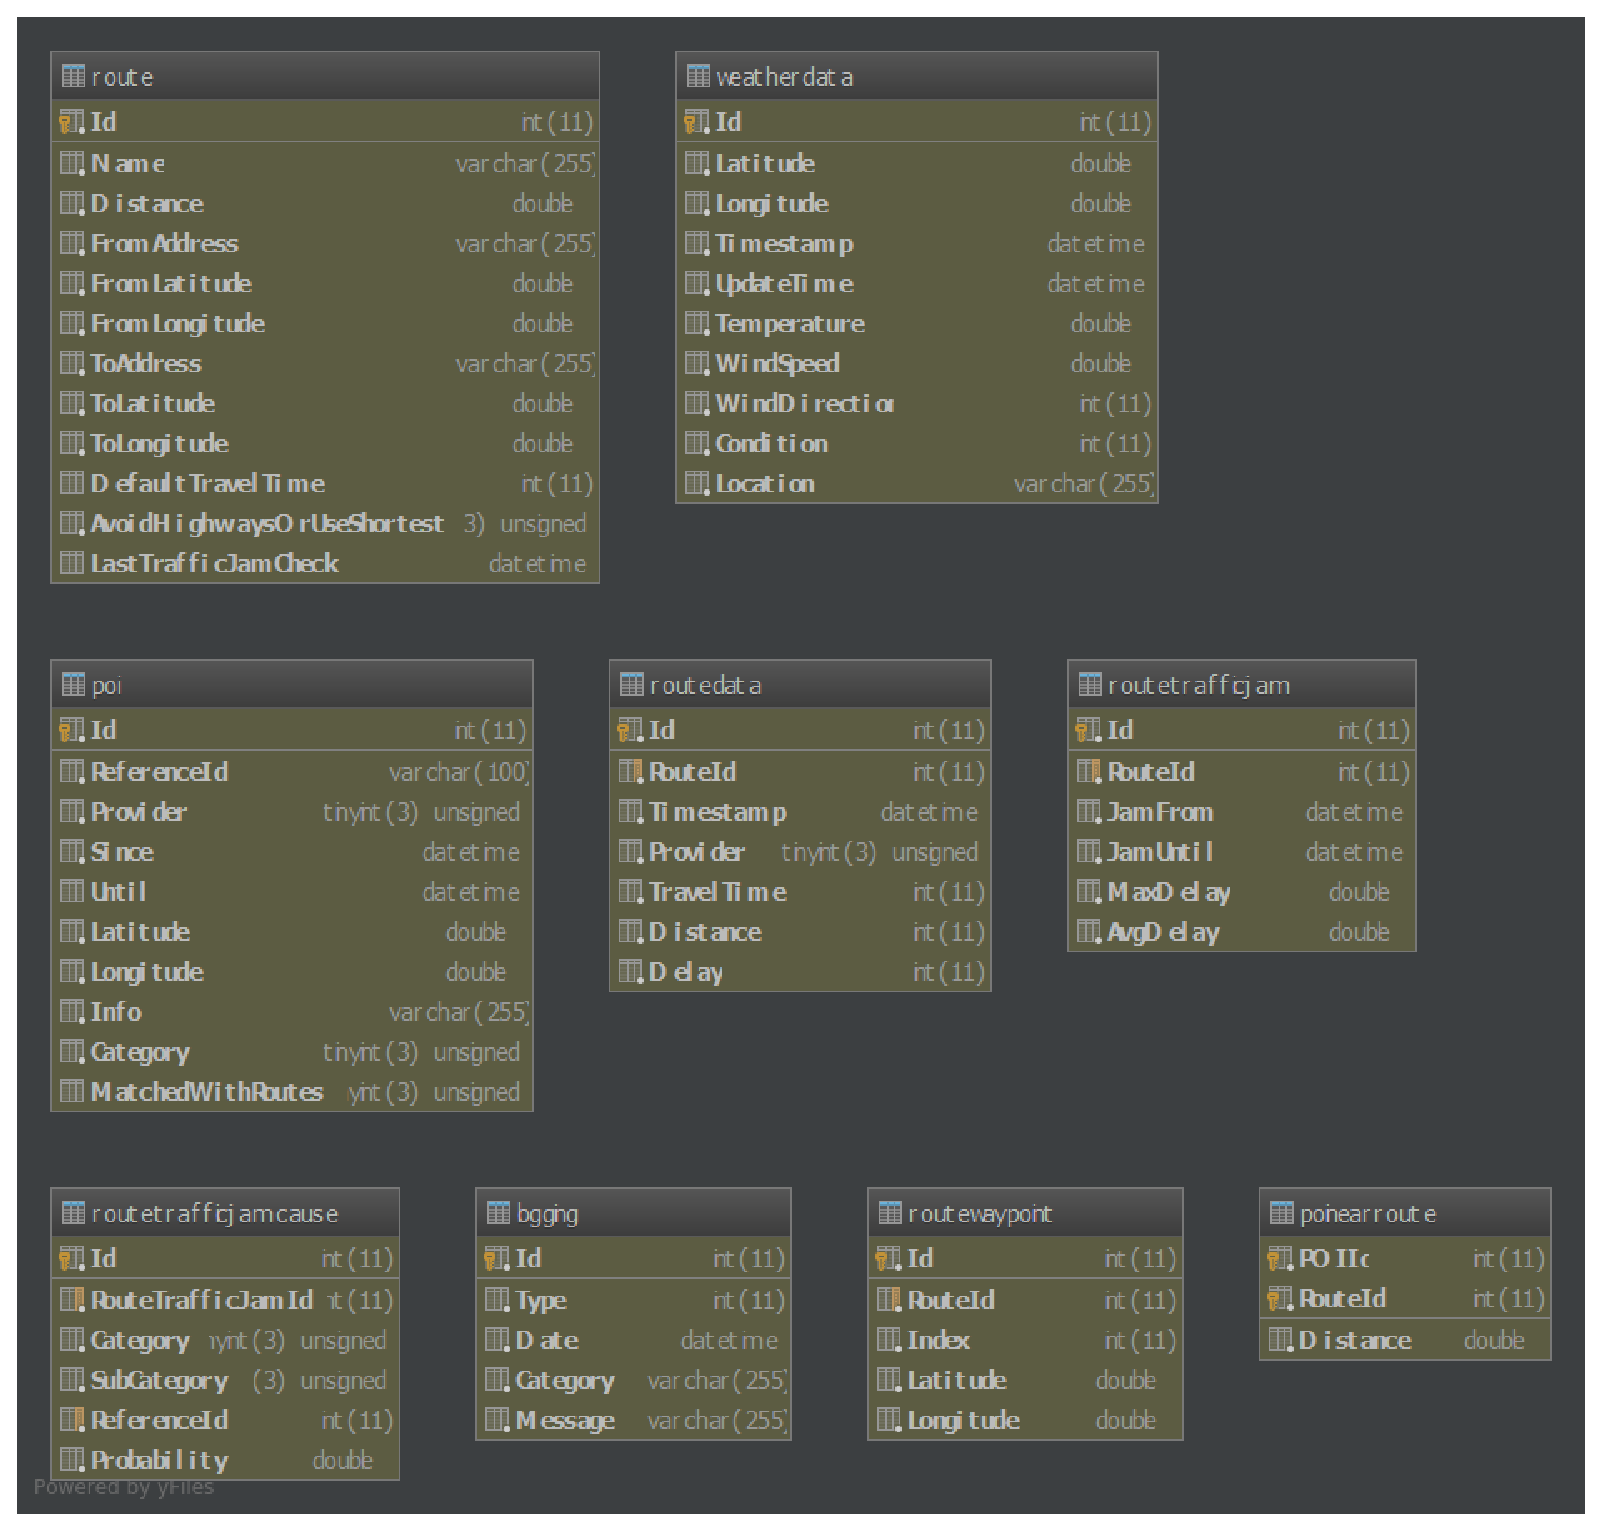
\includegraphics[width=\textwidth]{images/erd.eps}\\
\caption{Diagram - ERD}
\end{figure}


\subsection{Sequentiediagram - Bepalen File en Oorzaak}

\begin{figure}[H]
\centering
\includegraphics[angle=90, scale=0.34]{images/TrafficJamAnalysis.png}\\
\caption{Diagram - Bepalen File en Oorzaak}
\end{figure}


\subsection{Sequentiediagram - Polling verkeersgegevens}

\begin{figure}[H]
\centering
\includegraphics[angle=90, scale=0.4]{images/PollServiceAPIcalls.png}\\
\caption{Diagram - Polling verkeersgegevens}
\end{figure}


\subsection{Sequentiediagram - Overview Routes}

\begin{figure}[H]
\centering
\includegraphics[angle=90, scale=0.4]{images/OverviewRoutes.png}\\
\caption{Diagram - Overview Routes}
\end{figure}

\newpage

\section{Feedback + Vragen en antwoorden}

WIP

%\subsection{Algemene feedback sprint 1} -> weg ?

\subsection{Team -> Klant}

\textbf{Hoe kunnen we best een betrouwbaarheid aan een provider toekennen op basis van de gegevens die we van verschillende providers opgeslagen hebben?}\\
Onbeantwoord.(Dit is ook een vraag die we onszelf stellen..)

\textbf{Hoever terug moet de gegevens bewaard worden? Weken, maanden, jaren, altijd?}\\
Onbeantwoord.

\textbf{Moet er ’s nachts ook even vaak gepollt worden? Met andere woorden zijn er momenten waarop we het systeem minder moeten belasten?}\\
Onbeantwoord.

\textbf{Hoe moeten we de kleuren voorstellen van routes? Vb. Op basis van de vertraging?}\\
Onbeantwoord.

\textbf{Moeten er nog wijzigingen gebeuren op de trajectdetailpagina?}\\
Onbeantwoord.

\textbf{Welke filters moeten toegepast kunnen worden op de trajectdetailpagina?}\\
Onbeantwoord. (Aanvulling/wijziging van huidige filters..)\\

\textbf{Welke grafieken moeten zeker aanwezig zijn?}\\
Onbeantwoord. (Aanvulling/wijziging van huidige grafieken..)\\

\textbf{Moet de applicatie meertalig zijn?}\\
Onbeantwoord.

\newpage

\subsection{Klant -> Team}

\textbf{Is het mogelijk waarden tussen verschillende providers die sterk afwijken aan te duiden?}\\

\textbf{Is het mogelijk trajecten met de grootste vertragingen bovenaan te zetten?}\\

\textbf{Kunnen de tijden worden weergeven in de vorm van minuten en seconden i.p.v. seconden.}\\


\subsection{Team -> Team}

\textbf{Technische details?}\\
\begin{multicols}{2}
\begin{itemize}
\item Java 8
\item Spring MVC
\item IDE: Netbeans/IntelliJ
\item MariaDb
\item Glassfish 4.11
\item Bootstrap
\item Highcharts 
\item Leaflet
\end{itemize}
\end{multicols}

\textbf{1 gezamenlijke database of ieder lokaal afzonderlijk?}\\
Iedereen werkt lokaal op zijn eigen database-instantie.\\

\textbf{Wat is de projectstructuur}\\
3-lagenstructuur. Enerzijds VerkeerWeb (frontend) en anderzijds VerkeerDomain, VerkeerDomainData en VerkeerDal (backend).\\

\newpage
\section{Kwaliteitscontrole}
\label{sec:kwaliteitscontrole}

In deze kwaliteitscontrole worden enkele testen beschreven. Deze rubriek somt als het ware de verschillende testplannen op. Er wordt telkens wat uitleg gegeven over de gebruikte aanpakt gevolgd door een beschrijving of een uitvoering van dergelijke test. 

\subsection{Overzicht Testplan}

De unit testen zullen vooral de business logica van de verschillende use cases testen op een mock data laag met testgegevens. Hierdoor zijn de testgegevens steeds hetzelfde en kan bij aanpassingen aan de services gemakkelijk geverifiëerd worden of er geen bugs geintroduceerd zijn.

De integration tests testen de verbinding met de database en de stabiele werking van het systeem in het algemeen. Ook hier wordt gebruik gemaakt van de main flows van de belangrijkse use cases.

Tenslotte testen de usability testen de algemene gebruiksvriendelijkheid van de applicatie, o.a of het voor een leek die niet vertrouwd is met het systeem vlug duidelijk is waar alles te vinden is en hoe gemakkelijk hij/zij het vindt om bepaalde gegevens op te vragen. Verder wordt er ook gekeken naar de performantie en responsiviteit van de applicatie door heel veel data in de databank te steken en te kijken of er geen vertragingen naar boven komen.

\subsection{Unit Tests}

Om zeker te zijn dat bepaalde algoritmes van het project correct werken, worden er unit testen aangemaakt. Om maximaal rendement uit de unit testen te halen, worden er geen triviale testen gemaakt voor bijvoorbeeld setters zonder logica. Er zal gebruik gemaakt worden van het framework Mockito om dependecies te mocken en JUnit voor de testen. 

De belangrijkste algoritmes die getest moeten worden zijn:

\begin{itemize}
\item Het detecteren van extreme providers op de detail page (door Aaron).
\item Het gemiddelde berekenen van een route over een bepaalde periode en enkel voor bepaalde providers (door Aaron).
\item Het detecteren van files (door Dwight).
\end{itemize}

\subsection{Integration Tests (via Selenium)}

Het is een discussiepunt om de functionele acceptatie-testen van selenium nu al dan niet te categoriseren onder integratietesten. Omdat de testen toch wel data van backend ophalen via de frontend alsof ze een gebruiker zijn hebben we toch gekozen om deze hier te plaatsen. Een correctere term is waarschijnlijk smoke of sanity test.

Selenium IDE is een plugin waarmee je browseractiviteiten kan opnemen. Men kan elementen op de webapplicatie selecteren en deze controleren. Na het opnemen kan zo'n test case (of suite) geëxporteerd worden naar testen die uitgevoerd kunnen worden in bijvoorbeeld JUnit.

Een voorbeeld van zo'n test is het ophalen en controleren (via regex momenteel) of elke route wel een acceptabele normale reistijd, huidige reistijd en vertraging heeft. 

Een demo en voorbeeld zijn te zien op \url{https://www.youtube.com/watch?v=8HOH1TDGWdo}.

\subsection{Usability Tests (Use case testing)}

Met use case testing bedoelt men soms het ``het maken van'' use cases in een Agile of TDD (Test Driven Development)-omgeving. In deze rubriek hebben we echter de use cases genomen en deze omgezet in een stappenplan. Het doornemen van deze stappen test zo onze applicatie aan onze use cases. Op die manier worden de gewenste doelstelling getest en worden ook de use cases deel van de documentatie van het eindproduct.

Bij het maken van het stappenplan hebben we geprobeerd alles te schrijven vanuit de gebruike zijn standpunt. Om die reden zijn er enkele use cases die niet (rechtstreeks) getest kunnen worden door de gebruiker. Men zou alternatieven kunnen voorzien maar dit is niet echt nodig. In deze use cases worden alle gegevens verzamelt en weggeschreven naar de databank. Deze use cases zijn dan ook niet echt bedoelt om te testen in een usability test. SQL-queries of inloggen op de server en onze testscrips runnen zijn workarounds. Het is echter zo dat als de andere use case die getest worden aan de hand van usability tests (ook) gaan falen als deze use cases niet correct zijn. Daarom mogen we concluderen dat deze use cases correct doorloopbaar zijn zonder expliciet een stappenplan te volgen. 

\begin{itemize}
\item Uc: Verzamelen POI-gegevens
\item Uc: Verzamelen weergevens
\item Uc: Verzamel reistijdgegevens
\end{itemize}

Volgende 2 tabellen toont het stappenplan die opgemaakt werd op basis van de use cases. We doorlopen het stap voor stap een\, \cmark \, toont aan dat alles geslaagd is terwijl een\, \xmark \, aantoont dat er nog iets niet in orde is.

\begin{table}[H]
\centering
\begin{tabular}{|r|l|l|}
\hline
\multicolumn{3}{|c|}{{\textbf{UC: Bekijk routeoverzicht}}}                         \\ \hline
\multicolumn{1}{|c|}{Stappenplan:} &                                            &  \\ \hline
1.                                 & Gebruiker gaat naar de website.            & \cmark \\ \hline
2.                                 & Gebruiker kan op routeoverzicht klikken.   & \cmark \\ \hline
3.                                 & Een overzicht van de routes wordt getoond. & \cmark \\ \hline
4.                                 & Een overzicht van de routes wordt getoond. & \cmark \\ \hline
\multicolumn{3}{|c|}{{\textbf{UC: Bekijk routedetail}}}                            \\ \hline
\multicolumn{1}{|c|}{Stappenplan:} &                                            &  \\ \hline
1.                                 & Gebruiker gaat naar de website.            & \cmark \\ \hline
2.                                 & Gebruiker kan op routeoverzicht klikken.   & \cmark \\ \hline
3.                                 & Gebruiker kan op een route klikken voor de details. & \cmark \\ \hline
4.                                 & De routedetails worden getoond.            & \cmark \\ \hline
\multicolumn{3}{|c|}{{\textbf{UC: Bekijk routemap}}}                          \\ \hline
\multicolumn{1}{|c|}{Stappenplan:} &                                            &  \\ \hline
1.                                 & Gebruiker gaat naar de website.            & \cmark \\ \hline
2.                                 & Gebruiker kan op routemap klikken.   & \cmark \\ \hline
3.                                 & De routemap wordt getoond.        & \cmark \\ \hline
\multicolumn{3}{|c|}{{\textbf{UC: Vergelijk providerdata}}}                            \\ \hline
\multicolumn{1}{|c|}{Stappenplan:} &                                            &  \\ \hline
1.                                 & Gebruiker gaat naar de website.            & \cmark \\ \hline
2.                                 & Gebruiker kan op routeoverzicht klikken.   & \cmark \\ \hline
3.                                 & Gebruiker kan op een route klikken voor de details. & \cmark \\ \hline
4.                                 & Gebruiker kan providerdata vergelijken.            & \cmark \\ \hline
\multicolumn{3}{|c|}{{\textbf{UC: Wijzig route}}}                            \\ \hline
\multicolumn{1}{|c|}{Stappenplan:} &                                            &  \\ \hline
1.                                 & Gebruiker gaat naar de website.            & \cmark \\ \hline
2.                                 & Gebruiker kan op routeoverzicht klikken.   & \cmark \\ \hline
3.                                 & Gebruiker kan op wijzig klikken. & \cmark \\ \hline
4.                                 & Gebruiker kan de details van de route wijzigen.            & \cmark \\ \hline
\multicolumn{3}{|c|}{{\textbf{UC: Logpagina bekijken}}}                            \\ \hline
\multicolumn{1}{|c|}{Stappenplan:} &                                            &  \\ \hline
1.                                 & Gebruiker gaat naar de website.            & \cmark \\ \hline
2.                                 & Gebruiker kan op logpagina klikken.   & \xmark \\ \hline
\end{tabular}
\caption{Usability Tests (use case testing (1/2)}
\end{table}

\begin{table}[H]
\centering
\begin{tabular}{|r|l|l|}
\hline
\multicolumn{3}{|c|}{{\textbf{UC: Dashboard bekijken}}}                         \\ \hline
\multicolumn{1}{|c|}{Stappenplan:} &                                            &  \\ \hline
1.                                 & Gebruiker gaat naar de website.            & \cmark \\ \hline
2.                                 & Gebruiker kan dashboard(s) bekijken.       & \cmark \\ \hline
\multicolumn{3}{|c|}{{\textbf{UC: Aanbieden routegegevens met reistijden.}}}                            \\ \hline
\multicolumn{1}{|c|}{Stappenplan:} &                                            &  \\ \hline
1.                                 & Gebruiker maakt een specifieke request.            & \xmark \\ \hline
2.                                 & De gebruiker krijgt correcte gegevens naar gelang de request.   & \xmark \\ \hline
\multicolumn{3}{|c|}{{\textbf{UC: Vergelijk routes}}}                          \\ \hline
\multicolumn{1}{|c|}{Stappenplan:} &                                            &  \\ \hline
1.                                 & Gebruiker gaat naar de website.            & \xmark \\ \hline
2.                                 & Gebruiker klikt op vergelijk routes.   & \xmark \\ \hline
3.                                 & Gebruiker geeft routedetails op.       & \xmark \\ \hline
4.                                 & Een grafiek wordt getoond waarin de routes vergeleken kunnen worden.       & \xmark \\ \hline
\end{tabular}
\caption{Usability Tests (use case testing (2/2)}
\end{table}

Bovenstaande stappen werden overlopen op 16 april. Alle zaken die falen zijn nog geplande, niet-geïmplementeerde features. 


\subsection{Usability Tests (scenario)}


Deze manueel uitgevoerde scenarios dienen de usability and user experience (UX) te testen. Er werd aan 3 personen gevraagd om een specifiek scenario door te nemen. De testpersonen moeten aanduiden of ze de verschillende stappen van het scenario goed kunnen uitvoeren of niet, alsook het loggen van de gespendeerde tijd. Het uitvoeren van de verschillende stappen test als gevolg het gebruik van de applicatie. Tot slot werd er gevraagd aan de testpersonen of ze nog opmerkingen, vragen of onduidelijkheden hadden.

Er werd geopteerd om 3 profielen te benaderen. Onze keuze is uitgegaan naar een IT-deskundige en 2 niet-IT-deskundigen. Deze laatste groep verschilt dan nog eens in leeftijd (enederzijds $\pm 20$ jaar en anderzijds  $\pm 50$ jaar).

Er is 1 use case die we zelf uitvoerig gebruikt (en dus getest hebben) en dat is ``route wijzigen''. Het sprekt ook voor zich dat we op de productieomgeving deze use case liever niet laten derden doornemen door derden. ``De vergelijk routes''-use case is bovendien nog niet geïmplementeerd.

% Dit is getest en in orde:
% Ik kan een route wijzigen.

% Not implemented yet:

% Setting pagina
% Compare pagina
% Bij het invoeren van een verkeerde url op domein krijg ik een correcte errorpagina.

\newpage

\subsubsection{Template}

Het scenario (of stappenplan) dat werd gegeven aan de testpersonen ziet er als volgt uit:

\begin{table}[H]
\centering
\begin{tabular}{|r|l|l|l|l|l|}
\hline
\multicolumn{1}{|c|}{\textit{\textbf{Stap}}} & \multicolumn{1}{c|}{\textit{\textbf{Beschrijving}}}                                                                    & \multicolumn{1}{c|}{\textit{\textbf{Ok}}} & \multicolumn{1}
{c|}{\textit{\textbf{Ind.}}} & \multicolumn{1}
{c|}{\textit{\textbf{Cum.}}} \\ \hline
1 & \multicolumn{1}{p{9cm}|}{Ik kan naar de website: \url{http://verkeer-4.vop.tiwi.be/} surfen en inloggen met de credentials guest/1RRBpmM0KC.} & \multicolumn{1}{c|}{}                         &  &  \\ \hline

2 & \multicolumn{1}{p{9cm}|}{Ik kan het weer aflezen van de website.} & \multicolumn{1}{c|}{}     
&  &  \\ \hline

3 & \multicolumn{1}{p{9cm}|}{Ik kan de laatste tweets van ``VerkeerGentB'' zien.} & \multicolumn{1}{c|}{}   
&  &  \\ \hline

4 & \multicolumn{1}{p{9cm}|}{Ik kan een overzicht van alle routes zien met hun afstanden, standaardtijden, huidige reistijden en huidige vertragingen.} & \multicolumn{1}{c|}{}      
&  &  \\ \hline

5 & \multicolumn{1}{p{9cm}|}{Ik kan naar een route gaan en zijn weg visueel zien op een kaart.} & \multicolumn{1}{c|}{}      
&  &  \\ \hline

6 & \multicolumn{1}{p{9cm}|}{Ik kan de vertraging van Bing op Paryslaan (R4) northbound te weten komen.} & \multicolumn{1}{c|}{}      
&  &  \\ \hline

7 & \multicolumn{1}{p{9cm}|}{Ik kan een visueel overzicht krijgen op de kaart waar er momenteel vertragingen zijn.} & \multicolumn{1}{c|}{}      
&  &  \\ \hline

8 & \multicolumn{1}{p{9cm}|}{Ik kan visueel zien of er zich ergens probleempunten vertonen in de buurt van Gent.} & \multicolumn{1}{c|}{}      
&  &  \\ \hline

9 & \multicolumn{1}{p{9cm}|}{Ik kan te weten komen wat de huidige reistijd was per provider op 17 maart tussen 6:00 en 11:00 in de Rooigemlaan (R40) northbound.} & \multicolumn{1}{c|}{}      
&  &  \\ \hline

10 & \multicolumn{1}{p{9cm}|}{Ik kan te weten komen wat de vertraging was per provider op 17 maart tussen 6:00 en 11:00 in de Rooigemlaan (R40) northbound.} & \multicolumn{1}{c|}{}      
&  &  \\ \hline

11 & \multicolumn{1}{p{9cm}|}{Ik kan de data van vorige test opslaan als in een csv-bestand (te openen met excel).} & \multicolumn{1}{c|}{}      
&  &  \\ \hline

12 & \multicolumn{1}{p{9cm}|}{Ik kan te weten komen welke route volgens google het meeste vertraging heeft.} & \multicolumn{1}{c|}{}      
&  &  \\ \hline

13 & \multicolumn{1}{p{9cm}|}{Ik kan te weten komen welke route de grootste afstand heeft.} & \multicolumn{1}{c|}{}      
&  &  \\ \hline

\end{tabular}
\caption{Scenario Usability Test Template}
\end{table}


\subsubsection{Persoon 1: IT-deskundige}

\begin{table}[H]
\centering
\begin{tabular}{|r|l|l|l|l|}
\hline
\multicolumn{1}{|c|}{\textit{\textbf{Stap}}} & \multicolumn{1}{c|}{\textit{\textbf{Beschrijving}}}                                                                    & \multicolumn{1}{c|}{\textit{\textbf{Ok}}} & \multicolumn{1}
{c|}{\textit{\textbf{Ind.}}} & \multicolumn{1}
{c|}{\textit{\textbf{Cum.}}} \\ \hline
1 & \multicolumn{1}{p{9cm}|}{Ik kan naar de website: \url{http://verkeer-4.vop.tiwi.be/} surfen en inloggen met de credentials guest/1RRBpmM0KC.} & \multicolumn{1}{c|}{\cmark}                         & 00:30 & 00:30 \\ \hline

2 & \multicolumn{1}{p{9cm}|}{Ik kan het weer aflezen van de website.} & \multicolumn{1}{c|}{\cmark}     
& 00:05 & 00:35 \\ \hline

3 & \multicolumn{1}{p{9cm}|}{Ik kan de laatste tweets van ``VerkeerGentB'' zien.} & \multicolumn{1}{c|}{\cmark}   
& 00:00 & 00:35  \\ \hline

4 & \multicolumn{1}{p{9cm}|}{Ik kan een overzicht van alle routes zien met hun afstanden, standaardtijden, huidige reistijden en huidige vertragingen.} & \multicolumn{1}{c|}{\cmark}      
& 01:00 & 01:35  \\ \hline

5 & \multicolumn{1}{p{9cm}|}{Ik kan naar een route gaan en zijn weg visueel zien op een kaart.} & \multicolumn{1}{c|}{\cmark}      
& 01:00 & 02:35  \\ \hline

6 & \multicolumn{1}{p{9cm}|}{Ik kan de vertraging van Bing op Paryslaan (R4) northbound te weten komen.} & \multicolumn{1}{c|}{\cmark}      
& 02:00 & 04:35  \\ \hline

7 & \multicolumn{1}{p{9cm}|}{Ik kan een visueel overzicht krijgen op de kaart waar er momenteel vertragingen zijn.} & \multicolumn{1}{c|}{\cmark}      
& 01:00 & 05:35  \\ \hline

8 & \multicolumn{1}{p{9cm}|}{Ik kan visueel zien of er zich ergens probleempunten vertonen in de buurt van Gent.} & \multicolumn{1}{c|}{\cmark}      
& 00:00 & 05:35  \\ \hline

9 & \multicolumn{1}{p{9cm}|}{Ik kan te weten komen wat de huidige reistijd was per provider op 17 maart tussen 6:00 en 11:00 in de Rooigemlaan (R40) northbound.} & \multicolumn{1}{c|}{\cmark}      
& 02:00 & 07:35  \\ \hline

10 & \multicolumn{1}{p{9cm}|}{Ik kan te weten komen wat de vertraging was per provider op 17 maart tussen 6:00 en 11:00 in de Rooigemlaan (R40) northbound.} & \multicolumn{1}{c|}{\cmark}      
& 01:00 & 08:35  \\ \hline

11 & \multicolumn{1}{p{9cm}|}{Ik kan de data van vorige test opslaan als in een csv-bestand (te openen met excel).} & \multicolumn{1}{c|}{\cmark}      
& 00:05 & 08:40  \\ \hline

12 & \multicolumn{1}{p{9cm}|}{Ik kan te weten komen welke route volgens google het meeste vertraging heeft.} & \multicolumn{1}{c|}{\cmark}      
& 02:00 & 10:40  \\ \hline

13 & \multicolumn{1}{p{9cm}|}{Ik kan te weten komen welke route de grootste afstand heeft.} & \multicolumn{1}{c|}{\cmark}      
& 00:10 & 10:50  \\ \hline

\end{tabular}
\caption{Scenario Usability Test Persoon 1: IT-deskundige}
\end{table}

Opmerkingen:

\begin{itemize}
\item Onduidelijk navigatiemenu.
\item In het algemeen niet zo duidelijk als je niet doorklikt.
\item Zaken die nog niet geïmplementeerd zijn moeten er best nog niet op.
\end{itemize}

\subsubsection{Persoon 2: niet-IT-deskundige (1)}

\begin{table}[H]
\centering
\begin{tabular}{|r|l|l|l|l|}
\hline
\multicolumn{1}{|c|}{\textit{\textbf{Stap}}} & \multicolumn{1}{c|}{\textit{\textbf{Beschrijving}}}                                                                    & \multicolumn{1}{c|}{\textit{\textbf{Ok}}} & \multicolumn{1}
{c|}{\textit{\textbf{Ind.}}} & \multicolumn{1}
{c|}{\textit{\textbf{Cum.}}} \\ \hline
1 & \multicolumn{1}{p{9cm}|}{Ik kan naar de website: \url{http://verkeer-4.vop.tiwi.be/} surfen en inloggen met de credentials guest/1RRBpmM0KC.} & \multicolumn{1}{c|}{\cmark}                         & 00:40 & 00:40 \\ \hline

2 & \multicolumn{1}{p{9cm}|}{Ik kan het weer aflezen van de website.} & \multicolumn{1}{c|}{\cmark}     
& 00:05 & 00:45 \\ \hline

3 & \multicolumn{1}{p{9cm}|}{Ik kan de laatste tweets van ``VerkeerGentB'' zien.} & \multicolumn{1}{c|}{\cmark}   
& 00:00 & 00:45 \\ \hline

4 & \multicolumn{1}{p{9cm}|}{Ik kan een overzicht van alle routes zien met hun afstanden, standaardtijden, huidige reistijden en huidige vertragingen.} & \multicolumn{1}{c|}{\cmark}      
& 01:00 & 01:45 \\ \hline

5 & \multicolumn{1}{p{9cm}|}{Ik kan naar een route gaan en zijn weg visueel zien op een kaart.} & \multicolumn{1}{c|}{\cmark}      
& 00:30 & 02:15 \\ \hline

6 & \multicolumn{1}{p{9cm}|}{Ik kan de vertraging van Bing op Paryslaan (R4) northbound te weten komen.} & \multicolumn{1}{c|}{\cmark}      
& 01:00 & 03:15 \\ \hline

7 & \multicolumn{1}{p{9cm}|}{Ik kan een visueel overzicht krijgen op de kaart waar er momenteel vertragingen zijn.} & \multicolumn{1}{c|}{\cmark}      
& 01:00 & 04:15 \\ \hline

8 & \multicolumn{1}{p{9cm}|}{Ik kan visueel zien of er zich ergens probleempunten vertonen in de buurt van Gent.} & \multicolumn{1}{c|}{\cmark}      
& 00:00 & 04:15 \\ \hline

9 & \multicolumn{1}{p{9cm}|}{Ik kan te weten komen wat de huidige reistijd was per provider op 17 maart tussen 6:00 en 11:00 in de Rooigemlaan (R40) northbound.} & \multicolumn{1}{c|}{\cmark}      
& 01:30 & 05:45 \\ \hline

10 & \multicolumn{1}{p{9cm}|}{Ik kan te weten komen wat de vertraging was per provider op 17 maart tussen 6:00 en 11:00 in de Rooigemlaan (R40) northbound.} & \multicolumn{1}{c|}{\xmark}      
& 02:00 & 07:45 \\ \hline

11 & \multicolumn{1}{p{9cm}|}{Ik kan de data van vorige test opslaan als in een csv-bestand (te openen met excel).} & \multicolumn{1}{c|}{\cmark}      
& 00:30 & 08:15 \\ \hline

12 & \multicolumn{1}{p{9cm}|}{Ik kan te weten komen welke route volgens google het meeste vertraging heeft.} & \multicolumn{1}{c|}{\xmark}      
& 02:00 & 10:15 \\ \hline

13 & \multicolumn{1}{p{9cm}|}{Ik kan te weten komen welke route de grootste afstand heeft.} & \multicolumn{1}{c|}{\cmark}      
& 00:30 & 10:45 \\ \hline

\end{tabular}
\caption{Scenario Usability Test Persoon 2: niet-IT-deskundige (1)}
\end{table}

Opmerkingen:

\begin{itemize}
\item Bij het weer wordt niet aangegeven dat dit van Gent is.
\item CTT en D is niet duidelijk voor personen die er niet mee bezig zijn.
\item Er zou een duidelijkere scheiding moeten zijn tussen de providers vanboven omdat het niet duidelijk is welke CTT en D bij welke provider horen.
\item Sorteren niet duidelijk.
\end{itemize}

\subsubsection{Persoon 3: niet-IT-deskundige (2)}

\begin{table}[H]
\centering
\begin{tabular}{|r|l|l|l|l|}
\hline
\multicolumn{1}{|c|}{\textit{\textbf{Stap}}} & \multicolumn{1}{c|}{\textit{\textbf{Beschrijving}}}                                                                    & \multicolumn{1}{c|}{\textit{\textbf{Ok}}} & \multicolumn{1}
{c|}{\textit{\textbf{Ind.}}} & \multicolumn{1}
{c|}{\textit{\textbf{Cum.}}} \\ \hline
1 & \multicolumn{1}{p{9cm}|}{Ik kan naar de website: \url{http://verkeer-4.vop.tiwi.be/} surfen en inloggen met de credentials guest/1RRBpmM0KC.} & \multicolumn{1}{c|}{\cmark}                         & 01:40 & 01:40 \\ \hline

2 & \multicolumn{1}{p{9cm}|}{Ik kan het weer aflezen van de website.} & \multicolumn{1}{c|}{\cmark}     
& 00:10 & 01:50 \\ \hline

3 & \multicolumn{1}{p{9cm}|}{Ik kan de laatste tweets van ``VerkeerGentB'' zien.} & \multicolumn{1}{c|}{\cmark}   
& 00:10 & 02:00 \\ \hline

4 & \multicolumn{1}{p{9cm}|}{Ik kan een overzicht van alle routes zien met hun afstanden, standaardtijden, huidige reistijden en huidige vertragingen.} & \multicolumn{1}{c|}{\cmark}      
& 01:00 & 03:00 \\ \hline

5 & \multicolumn{1}{p{9cm}|}{Ik kan naar een route gaan en zijn weg visueel zien op een kaart.} & \multicolumn{1}{c|}{\cmark}      
& 00:30 & 03:30 \\ \hline

6 & \multicolumn{1}{p{9cm}|}{Ik kan de vertraging van Bing op Paryslaan (R4) northbound te weten komen.} & \multicolumn{1}{c|}{\cmark}      
& 02:00 & 05:30 \\ \hline

7 & \multicolumn{1}{p{9cm}|}{Ik kan een visueel overzicht krijgen op de kaart waar er momenteel vertragingen zijn.} & \multicolumn{1}{c|}{\cmark}      
& 01:00 & 06:30 \\ \hline

8 & \multicolumn{1}{p{9cm}|}{Ik kan visueel zien of er zich ergens probleempunten vertonen in de buurt van Gent.} & \multicolumn{1}{c|}{\cmark}      
& 00:10 & 06:40 \\ \hline

9 & \multicolumn{1}{p{9cm}|}{Ik kan te weten komen wat de huidige reistijd was per provider op 17 maart tussen 6:00 en 11:00 in de Rooigemlaan (R40) northbound.} & \multicolumn{1}{c|}{\cmark}      
& 02:30 & 09:10 \\ \hline

10 & \multicolumn{1}{p{9cm}|}{Ik kan te weten komen wat de vertraging was per provider op 17 maart tussen 6:00 en 11:00 in de Rooigemlaan (R40) northbound.} & \multicolumn{1}{c|}{\xmark}      
& 02:30 & 11:40 \\ \hline

11 & \multicolumn{1}{p{9cm}|}{Ik kan de data van vorige test opslaan als in een csv-bestand (te openen met excel).} & \multicolumn{1}{c|}{\cmark}      
& 01:00 & 12:40 \\ \hline

12 & \multicolumn{1}{p{9cm}|}{Ik kan te weten komen welke route volgens google het meeste vertraging heeft.} & \multicolumn{1}{c|}{\xmark}      
& 02:30 & 15:10 \\ \hline

13 & \multicolumn{1}{p{9cm}|}{Ik kan te weten komen welke route de grootste afstand heeft.} & \multicolumn{1}{c|}{\cmark}      
& 01:00 & 16:10 \\ \hline

\end{tabular}
\caption{Scenario Usability Test Persoon 3: niet-IT-deskundige (2)}
\end{table}

Opmerkingen:

\begin{itemize}
\item CTT en D is niet duidelijk voor personen die er niet mee bezig zijn.
\item Er zou een duidelijkere scheiding moeten zijn tussen de providers vanboven omdat het niet duidelijk is welke CTT en D bij welke provider horen.
\item Sorteren niet duidelijk.
\item Opslaan is niet duidelijk aangegeven.
\end{itemize}



\newpage

\subsection{Load Tests (via Apache JMeter)}

% Algemene uitleg:

% Number of threats -> en loops (wij altijd 1 keer)

% Ramp-up needs to be long enough to avoid too large a work-load at the start of a test, and short enough that the last threads start running before the first ones finish (unless one wants that to happen).

Apache JMeter is een load testing tool waarin je users kan simuleren voor je webapplicatie. In de vorm van threads worden zo HTTP Requests uitgevoerd naar de verschillende pagina's. Op die manier kan men vrij snel een server testen tegen veel verkeer.

We hebben drie testen voorzien. De eerste bezoekt enkel de homepagina (en vult de basic auth correct in). De tweede gaat vervolgens nog naar de map view en de derde simuleert een volwaardige gebruiker die van het dashboard naar de overview surft om nadien een route te selecteren die hij in detail wil bekijken. De testen worden lokaal uitgevoerd tegen de productieserver. 

Een demo is te vinden in de vorm van een filmpje: \url{https://www.youtube.com/watch?v=h2HiMyBYgCI}.


\begin{figure}[H]
\centering
\includegraphics[width=\textwidth]{images/jmeterexample.png}\\
\caption{Apache JMeter - Voorbeeld}
\end{figure}









\newpage

\section{Technische handleiding}
\label{sec:technischehandleiding}

De applicatie is onderverdeeld in 3 lagen:
\begin{itemize}
\item De GUI layer: dit is de volledige MVC website met glassfish als server en bevat
  \begin{itemize}
  \item Controllers: de controllers beheren de HTTP acties, valideren de user input en roepen de overeenkomstige services uit het domain aan.
  \item Views: de views bestaan uit standaard JSP pages die met behulp van een model dat eraan meegegeven wordt in de controllers de html kan genereren.
  \item ViewModels: de gegevens die de controllers verzamelen van de domain services worden omgezet en indien nodig gecombineerd tot viewmodels die alle gegevens bevatten dat moet getoond worden in de pagina.
  \item DataObjects: voor ajax calls wordt er JSON teruggegeven die in de javascript code kan verwerkt worden. De json wordt automatisch gegenereerd van de data objecten die de controller teruggeeft. In feite zijn de view models en data objects gelijkaardig, de view models worden verwerkt aan server side, terwijl de data objects aan client side verwerkt worden.
  \item Shared Views: er zijn een aantal shared views voorzien zodat er geen html moet gecopy paste worden tussen meerdere views, zoals de inhoud van de head tag. Zodra html op meerdere views wordt gebruikt is het interessant om hiervoor een shared view te voorzien (met eventueel op te geven parameters zoals de title parameter in de head shared view).
  \item Javascript/Typescript: de code die aan client side uitgevoerd moet worden is deels geschreven in Typescript (een superset van javascript met een strong type system en transpiled naar javascript) en deels in plain javascript. De scripts zitten per pagina elk afzonderlijk in aparte bestanden die met script tags geinclude worden in de views.
  \item CSS: Er wordt gebruik gemaakt van Bootstrap als layout framework. Wanneer extra CSS moet toegepast worden op een pagina is hiervoor een apart stylesheet bestand voorzien die met een link tag wordt geinclude in de view.
  \end{itemize}
\item De Domain layer: de domain layer is opgesplitst in 2 delen:
  \begin{itemize}
  \item Domain: hierin zitten alle services die de business logic van de applicatie verwerken. De services maken gebruik van de domain objects. Voor elke service is een interface voorzien en hun bijhorende implementatie, hierdoor kan later nog gebruik gemaakt worden van dependency injection om de services automatisch te construeren. Elke service erft over van de BaseService die de UnitOfWork instantie voorziet om de gegevens uit de DAL op te vragen. De services zijn ongeveer ingedeeld volgens business unit:
  	\begin{itemize}
    \item RouteService: de Route service beheert alles omtrent de routes zelf en zorgt dat routes kunnen opgevraagd worden met hun onderliggende data, waypoints en gedetecteerde files, kunnen geupdate worden
    
    \item ProviderService: de Provider service voorziet alle nodige implementatie om de route data van alle routes efficient te verzamelen van verschillende providers. Zowel de route data (vertraging, huidige reistijd, ..) als de POI's (incident, road closed, ...) worden met behulp van de verschillende geregistreerde providers opgevraagd. Alle providers zijn apart geimplementeerd in de sub package "provider" en implementeren naargelang de beschikbare functionaliteit de interfaces IProvider (route data van 1 route opvragen), ISummaryProvider (route data van alle routes in 1x opvragen), IPOIProvider (poi's opvragen binnen een bounding box), IWeatherProvider (weergegevens opvragen rondom de routes). Sommige providers maken gebruik van een API die aangesproken wordt, andere maken gebruik van perl scrape scripts die de gevraagde gegevens teruggeven. Als beide beschikbaar zijn wordt steeds de scrape scripts eerst uitgeprobeerd, hierdoor wordt er geen verbruik om de API keys geregistreerd.
    
    \item POIService: de POI Service zorgt voornamelijk voor het opslaan en opvragen van POI's binnen een regio en bepaalde periode. De service kan ook de POI's matchen met nearby routes zodat POI's steeds voor éénbepaalde route kan opgevraagd worden.
    
    \item WeatherService: de Weather service voorziet methodes om de opvraagde weergegevens op te slaan in de databank en terug op te vragen.
    \end{itemize}
  
  \item Domain Objects: dit zijn alle data objecten die gebruikt worden en zijn ook de objecten die in de DAL layer worden gemapped naar tabels in de database. De volgende objecten worden momenteel gebruikt:
  	\begin{itemize}
    \item Route: stelt een route voor met basisgegevens als naam en start en eindpunt (in latitude en longitude). Verder is er nog een flag dat aangeeft of routes moeten berekend worden als snelste of eerder als kortste (of avoid highways). Dit is nodig voor bepaalde routes die anders de autostrade zouden kiezen terwijl dat niet gewenst is.
    \item RouteData: route data is een data punt verzameld van een specifieke provider op een bepaald tijdstip en bevat de reistijd en vertraging. De afstand van de route wordt ook mee bijgehouden zodat kan gedetecteerd worden of de provider een alternatieve route heeft voorgesteld ipv de gewenste route.
    \item RouteWaypoint: elke route is van de start tot einde onderverdeeld in segmenten. Een route waypoint is zo een tussenliggend punt en bevat enkel de geografische coordinaten. Waypoints worden berekend bij het wijzigen van de start/eind positie van een route en worden gebruikt bij het tonen van de route op een kaart en bij de controle of POI dicht bij een route ligt
    \newline
    \item POI: stelt een gebeurtenis voor op een bepaald punt en heeft een tijdsperiode wanneer de POI actief door de provider werd voorgesteld, de Until wordt pas ingevuld wanneer de POI niet meer wordt teruggegeven door de provider, dwz dat alle actieve POI's degene zijn met Until = NULL. POI's hebben ook een vaste categorielijst waartoe ze behoren, die op de website vertaald wordt naar de overeenkomstige icoontjes. De reference id van een POI is de unieke ID die de provider aan de POI gegeven heeft en wordt gebruikt om te detecteren bij opeenvolgende polls of het over dezelfde POI gaat of niet. Tenslotte bevat een POI ook nog een flag dat aangeeft of de POI reeds verwerkt is door de service die POI's matched met nearby routes.
    \item POINearRoute: POI's worden periodiek gematched met naburige routes. Dit object stelt zo een matching tussen een POI en een route voor.
    \newline
    \item RouteTrafficJam: elke dag wordt de data van alle routes geanalyseerd en worden file periodes opgespoord en deze periodes worden opgeslagen als dit object in de databank. Hierdoor moet de zware berekening maar éénmaal gebeuren en kan men nadien gewoon deze objecten raadplegen. Buiten de start en eind van de periode bevat het object ook nog een gemiddelde en maximum van de vertraging over de periode.
    \item RouteTrafficJamCause: voor elke file probeert de service ook oorzaken te zoeken wat de aanleiding zou geweest zijn, vb. accidenten die actief waren aan de start van de file is een goede kandidaat. Elke oorzaak wordt opgeslagen als een ROuteTrafifcJamCause object met een waarschijnlijkheidskans. Een oorzaak heeft een categorie (POI, Weer,..) en een subcategorie dat de categorie van bvb de POI zelf mee opslaat. Hierdoor kan er efficient een overzicht getrokken worden van alle files met hun oorzaken.
    \newline
    \item WeatherData: dit object bevat de weergegevens op een bepaald tijdstip en kan zo mee opgenomen worden als oorzaak bij files (vb mist of zware regenbui).
    \end{itemize}
  \end{itemize}
De domain data bevat ook nog een aantal "composite" of samengestelde objecten die door JOINs in de database werden gecombineerd, vb POIWithDistanceToRoute is een POI object maar bevat nog een extra veld afstand dat door een join met POINearRoute is gecombineerd.

\item De DAL layer: de DAL layer bevat de repositories (DbSet<T> klassen) van alle domain objecten om en voorzien standaard methodes voor de CRUD van de objecten. Als er specifieke gegevens moeten worden opgevraagd of extra filters moeten toegepast worden kan de repository van een object overgeerft worden en kan daarin de extra functionaliteit in worden voorzien. Om de applicatie efficient te houden is het nuttig om de joins reeds op de database uit te voeren en de gecombineerde gegevens terug te geven naar de domain services ipv de gegevens manueel in code te combineren.
\newline
Alle repositories zijn opvraagbaar via een overkoepeld UnitOfWork object dat ook opgesplitst is in een interface en implementatie. Hierdoor is het eenvoudiger de repositories te mocken voor unit testen en kan ook dependency injection gebruikt worden om in één keer de volledige DAL te initializeren.
\newline
De database wordt aangesproken met een micro ORM Sql2o. Deze library zorgt ervoor dat objecten kunnen vertaald worden naar parameters in de SQL queries en dat de dataset dat teruggegeven wordt automatisch vertaald wordt naar objecten. Aangezien we na verloop van tijd met veel data werken (miljoenen rijen) hebben we de overhead van de ORM zoveel mogelijk beperkt. Hibernate is gemakkelijk 10x trager dan Sql2o, dat maar een fractie trager is dan het manueel mappen van gegevens op de objecten.

\end{itemize}

Buiten de standaard 3-tier structuur is er ook nog een extra console applicatie voorzien dat periodiek verschillende acties uitvoert. Elke actie wordt in een aparte service geimplementeerd en erft over van de BaseService klasse die de scheduling van de actie op zich neemt. Momenteel zijn de volgende acties gedefinieerd:
\begin{itemize}
\item DataScrapingService: (elke 5min) deze service polled voor alle routes de RouteData gegevens aan alle providers. Per route worden de poll acties in parallel uitgevoerd zodat er zo weinig mogelijk verschil in tijd zit tussen de verkregen waarden. De service verzamelt ook alle POI gegevens voor elke provider.
\item BackgroundPOIRouteMatcherService: (elke 5min) deze service gaat na welke POI's nog niet gematched zijn met naburige routes en zal deze gaan matchen. Hierdoor worden POINearbyRoute objecten aangemaakt en wordt nadien de POI matching status geupdate.
\item TrafficJamAnalysisService: (elke 24u) deze service bekijkt de gegevens van alle routes dag per dag en zal de file periodes met hun oorzaken achterhalen. Alleen dagen die reeds volledig in het verleden liggen komen in aanmerking, aangezien voor die dagen geen gegevens meer zullen wijzigen.
\item WeatherPollService: (elke 5min) deze service polled alle weer providers om de recentste weergegevens op te slaan.
\end{itemize}

De console applicatie draait momenteel in een screen sessie op de server, waardoor het mogelijk is de output gemakkelijk te bekijken.
\newpage

\section{Gebruikershandleiding}
\label{sec:gebruikershandleiding}

\subsection{Inleiding}
Dit is een handleiding geschreven als informatieve bron bij het gebruik van de website “Verkeer-4.vop.tiwi.be”. Het beoogt een overzicht te geven bij het opzoeken van verkeersinformatie in en rond Gent. Dit zowel realtime als in het verleden.

\subsection{Het Dashboard}
Bij het surfen naar “Verkeer-4.vop.tiwi.be” zal u verwezen worden naar het dashboard van de website. Hier kunt u een korte samenvatting vinden van de belangrijkste informatie rond verkeer. 

\begin{itemize}
\item \textbf{Status - Errors} geeft een overzicht van de recente gebeurtenissen rond de applicatie. Het geeft een beeld van wat er misloopt.
\item \textbf{POI Overview} biedt een overzicht van de huidige “Points Of Interest”.  Hier worden onder andere ongevallen, trajectcontroles en belangrijke evenementen aangehaald.
\item De \textbf{Minimap} zorgt voor een visuele weergave van de verkeersituatie in en rond Gent. Zowel de files als de POI’s worden weergeven.
\item De \textbf{Weather widget} wordt gebruikt om een korte schets van het weer in Gent te weergeven. Dit kan het verkeer namelijk sterk beïnvloeden.
\item De \textbf{Twitter Wall}  toont de recente gebeurtenissen in en rond Gent die werden gemeld door de stad Gent.
\end{itemize}

\begin{figure}[H]
\centering
\includegraphics[width=0.6\textwidth]{images/dashboard.png}\\
\caption{Handleiding - Dashboard}
\end{figure}

Om verder te gaan naar de detail pagina’s kunt u gebruik maken van de links aan de bovenkant van de pagina.
Zo is het mogelijk om een overzicht te krijgen van de verschillende routes in de stad Gent. Ook een weergave op kaart en vergelijking tussen verschillende routes is mogelijk.

\subsection{Overview}

Bovenaan de pagina \textbf{“Overview”} kan u kiezen uit de tabbladen: \textbf{“Summary”} , \textbf{“For each provider”} en “By route”.

\begin{figure}[H]
\centering
\includegraphics[width=\textwidth]{images/overview.png}\\
\caption{Handleiding - Overview}
\end{figure}

\subsubsection{Summary}

Het tabblad “Summary” geeft een samenvatting van de verschillende routes in beide richtingen. De belangrijkste data zoals naam (Name), afstand (Distance), standaard reisduur (Standard Travel Time), huidige tijdsduur (Current Travel Time) en vertraging (Delay) worden weergeven. Het is mogelijk te sorteren op een bepaald onderwerp door op de hoofding van de tabel te klikken. 

Afhankelijk van de opgelopen vertraging wordt een kleur toegekend aan elk traject. De kleur aanduiding varieert tussen groen (geen file) en rood (zware file).

De trajecten worden in beide richtingen weergeven. Dit wordt aangegeven door de windrichting waarin deze gelegen zijn. (East - West - North - South bound). Bij het klikken op een traject komt u terecht op de detail pagina voor dat traject.


\begin{figure}[H]
\centering
\includegraphics[width=0.75\textwidth]{images/summary.png}\\
\caption{Handleiding - Summary}
\end{figure}

Wijzigingen aan de routes kunnen gemaakt worden door bij een bepaalde route op Edit te klikken. Dit wordt hieronder verder beschreven.

\begin{figure}[H]
\centering
\includegraphics[width=0.75\textwidth]{images/edit.png}\\
\caption{Handleiding - Zoom in op Edit}
\end{figure}

\subsubsection{Detail per traject}

Op deze pagina vindt u de gedetailleerde informatie over het gekozen traject. 

\begin{itemize} 
\item Bovenaan worden de reistijden en vertragingen per provider weergeven. Aan de rechterkant staat het traject afgebeeld op een kaart met een visuele weergave van hoe het verkeer verloopt op dit traject.
\item Bij \textbf{Filteroptions} kan de begin- en einddatum geselecteerd worden als parameters voor het genereren van een grafiek. 
\item In \textbf{History} wordt de grafiek gegenereerd die de tijdsduur, om dit traject af te leggen, grafisch voorstelt tussen het interval ingesteld bij filteroptions.
\item \textbf{Traffic jams} geeft alle files die zijn opgevangen in dat bepaald interval. Zo wordt er weergeven hoe lang de file heeft geduurd (\textbf{Duration}), wat de gemiddelde vertraging (\textbf{Avg delay}) en piek vertraging (\textbf{Peak delay}) was en de mogelijke oorzaken (\textbf{Possible causes}) van de file. De mogelijke oorzaken kunnen invloeden zijn van ongevallen, werken of het weer.
\end{itemize}

\begin{figure}[H]
\centering
\includegraphics[width=0.75\textwidth]{images/detail.png}\\
\caption{Handleiding - Detail (1/2)}
\end{figure}

\begin{figure}[H]
\centering
\includegraphics[width=0.75\textwidth]{images/detail2.png}\\
\caption{Handleiding - Detail (2/2)}
\end{figure}

\subsubsection{Edit}

Op het tabblad \textbf{"Summary"} kunnen de trajecten aangepast worden via de knop \textbf{Edit}. Hier kunnen de \textbf{name}, \textbf{from}- en \textbf{to} positions van het traject aangepast worden. De start- en eindpositie kunnen op 2 manieren aangepast worden, door de positie in te geven in het tekstveld of door op het kaartje de rode pijl te verslepen via de rechtermuisknop. Klik na de aanpassingen onderaan op \textbf{Save}.

\begin{figure}[H]
\centering
\includegraphics[width=0.75\textwidth]{images/editRoute.png}\\
\caption{Handleiding - Aanpassen Route}
\end{figure}

\subsubsection{For each provider}

Op het tabblad \textbf{“For each provider”} worden de reistijd (\textbf{CTT, Current Travel Time}) en de vertraging (\textbf{D, Delay}) per traject en per verkeersprovider weergegeven. Via het tandwiel kan er worden om bepaalde providers tijdelijk uit te schakelen in het overzicht.

\textbf{Betekenis van de kolommen}
\begin{itemize} 
\item \textbf{Distance} geeft de afstand van het traject.
\item \textbf{Current Travel Time} wordt berekend door het gemiddelde te nemen over de huidige reistijden van de verschillende providers.
\item \textbf{Avg. Delay} geeft de gemiddelde vertraging voor alle providers.
\item \textbf{CCT} geeft de huidige reistijd per provider weer.
\item \textbf{D}  geeft de huidige vertraging per provider weer.
\end{itemize}

\begin{figure}[H]
\centering
\includegraphics[width=\textwidth]{images/forEachProvider.png}\\
\caption{Handleiding - For Each Provider}
\end{figure}

\subsubsection{By Route}

Op het tabblad “By route” word dezelfde data weergeven zoals bij “For each provider”, maar hier wordt de data gesorteerd per route.

\begin{figure}[H]
\centering
\includegraphics[width=0.9\textwidth]{images/byRoute.png}\\
\caption{Handleiding - By Route}
\end{figure}

\subsection{Map View}

Op de pagina \textbf{“Map View”} worden alle trajecten afgebeeld op een kaart. Afhankelijk van de opgelopen vertraging wordt een kleur toegekend aan elk traject. Het traject wordt aangeduid met een bewegende route waardoor het duidelijk wordt in welke richting het verkeer zich beweegt. Door een traject af te vinken wordt het niet meer weergegeven op de kaart.

\begin{figure}[H]
\centering
\includegraphics[width=\textwidth]{images/mapView.png}\\
\caption{Handleiding - Map View}
\end{figure}
\newpage

\section{Installatiehandleiding}
\label{sec:installatiehandleiding}

\subsection{Te installeren software}

Volgende handleiding heeft de software gedeployed op een ubuntu distributie. Elk systeem (of distributie) die Glassfish, Java, Mariadb (of MySQL) en perl ondersteunt, kan gebruikt worden. De uitgevoerde commando's zullen echter verschillen. Werk je bijvoorbeeld op een centos of een fedora dan zal de apt-get packet manager niet werken en zal je yum moeten gebruiken.

Volgende zaken heb je nodig vanop je client systeem bij aanvang van de installatie:

\begin{itemize}
\item Terminal/console/putty/git bash die kan ssh'n naar de server.
\item Database dump in de vorm van een SQL-bestand (hier: verkeer.sql).
\item De pollservice die uitgevoerd wordt op de server (hier: verkeerPollService.jar)
\item De scrapers (hier: de map /scrapers/)
\item De webapplicatie die gedeployed wordt op glassfish (hier: verkeerweb.war)
\end{itemize}

Alle commando's die uitgevoerd opgesomd zijn, worden verondersteld uitgevoerd te worden op de ubuntu-server! Het SQL-bestand, de pollservice en de map /scrapers/ moeten op de server overgezet worden. Dit kan bijvoorbeeld via sftp of scp.

Een voorbeeld is:

\begin{lstlisting}[style=BashInputStyle]
	scp verkeer.sql root@x.y.z.q:/verkeer
	scp pollservice.jar root@x.y.z.q:/verkeer
	scp -r scrapers root@x.y.z.q:/verkeer/scrapers
\end{lstlisting}

\subsubsection{Datum/uur/tijdzone instellen}

\begin{lstlisting}[style=BashInputStyle]
	sudo timedatectl set-timezone Europe/Brussels
\end{lstlisting}

Een andere optie is via:

\begin{lstlisting}[style=BashInputStyle]
	apt-get install ntpdate
	dpkg-reconfigure tzdata
\end{lstlisting}





\subsubsection{Java 8 installeren}

\begin{lstlisting}[style=BashInputStyle]
	sudo add-apt-repository ppa:openjdk-r/ppa
	sudo apt-get update 
	sudo apt-get install openjdk-8-jdk -y
\end{lstlisting}

Controleren kan via:

\begin{lstlisting}[style=BashInputStyle]
	java -version
\end{lstlisting}

\subsubsection{Mariadb installeren}

\begin{lstlisting}[style=BashInputStyle]
	sudo apt-get install mariadb-server -y
\end{lstlisting}

Er zal gevraagd worden om een wachtwoord te kiezen voor mysql/mariadb.

\subsubsection{Extra tools installeren}

\begin{lstlisting}[style=BashInputStyle]
	sudo apt-get install unzip gcc make libjson-perl -y
\end{lstlisting}

Unzip gebruiken we om straks te unzippen. De c compiler, make hebben we nodig om de nodige zaken voor de scrapers te installeren.

\subsubsection{Glassfish installeren}

\begin{lstlisting}[style=BashInputStyle]
	wget http://download.oracle.com/glassfish/4.1/release/glassfish-4.1.zip
	unzip glassfish-4.1.1.zip -d /opt
	/opt/glassfish4/bin/asadmin start-domain
	/opt/glassfish4/bin/asadmin change-admin-password
	/opt/glassfish4/bin/asadmin enable-secure-admin
	/opt/glassfish4/bin/asadmin restart-domain
\end{lstlisting}

Met deze commando's doorloop je enkele stappen om een admin gebruiker te maken en het lege wachtwoord te wijzigen. Indien je vaak het asadmin programma gaat gebruiken dan kan het handig zijn om /opt/glassfish4/bin op te nemen in je PATH en dit toe te voegen aan je ~/.profile. Om een domein te stoppen gebruik je het commando ``asadmin stop-domain''.

\subsubsection{Perl installeren}

\begin{lstlisting}[style=BashInputStyle]
	sudo cpan JSON
	perl -MCPAN -e shell
		> install JSON::XS
\end{lstlisting}

\subsubsection{Mysql database verkeer in orde brengen}

\begin{lstlisting}[style=BashInputStyle]
	mysql -p
		create database verkeer;
		exit;
	mysql verkeer -u root < "verkeer.sql"
\end{lstlisting}

\subsubsection{Scrapers testen}

\begin{lstlisting}[style=BashInputStyle]
	root@server:~/scrapers# ./testscrapers.sh
\end{lstlisting}

Met dit scriptje worden alle scrapers getest. Op deze manier zien we of er data binnengehaald kan worden of niet.

\subsubsection{Poll service in een scriptje}

De poll service staat in dit voorbeeld in de root: /root/verkeerPollService.jar.
Met volgend script (runpollservice.sh) zorgen we ervoor dat hij automatisch herstart bij crashen:

\begin{lstlisting}[style=BashInputStyle]
	#!/bin/bash

	while true
	do
   		java -Xms256m -Xmx512m -jar VerkeerPollService.jar
  		#restart loop
   		sleep 5
	done
\end{lstlisting}

Het starten van de poll service gebeurt best in een screen:

\begin{lstlisting}[style=BashInputStyle]
	screen -S pollservice
	./runpollservice.sh
\end{lstlisting}

Met CTRL+A,D kan je het detachen.

\subsubsection{Instellen backup}

Volgende commando's voeren een script uit om een backup te maken aan de hand van een crontab.

\begin{lstlisting}[style=BashInputStyle]
	crontab -e
	#backup mysql db every midnight
	0 0 * * * /root/backupverkeer.sh
\end{lstlisting}

\subsubsection{Uploaden Verkeerweb}

Dit gebeurt in de browser door te surven naar glassfish. Deze is bereikbaar via http://server:4848. Inloggen doe je met de credentials die eerder werden ingesteld bij glassfish. Daarna kies je voor deploy application en kies je de war:

\begin{figure}[H]
\centering
\includegraphics[width=\textwidth]{images/uploadverkeerweb.png}\\
\caption{Uploaden Verkeerweb}
\end{figure}
\newpage

\subsection{Documentatie Scrapers}

De applicatie draait in een oneindige lus en zorgt ervoor dat elke 5min de poll methode wordt opgeroepen. In de poll service worden alle routes overlopen en per route alle providers in parallel opgeroepen. Hierdoor is het mogelijk om binnen de 7 sec alle gegevens voor een bepaalde route terug te krijgen. Er zijn momenteel 34 trajecten met max 7sec tussen, dus kan alles gepolled worden in 238sec, wat binnen de 5min valt. Hierdoor zijn we zeker dat de laatste gegevens elke 5min wordt opgevragen. \\ 

Er zijn 2 soorten providers om de route gegevens te bepalen:

\begin{itemize}
\item Providers van ISummaryProvider zoals Coyote geven alle routes in één keer terug, dat zorgt ervoor dat die maar éénmaal om de 5min moet opgeroepen worden.
\item Andere Providers van IProvider vragen gegevens op per route. Bijna alle providers maken onderliggend gebruik van perl scripts die met curl (commandline) de gegevens opvragen. Enkel Google Maps of Bing Maps is er geen scraper voorzien. Bij andere verschillende providers zoals TomTom en Here Maps is er een fallback naar de API met API keys die moeten geconfigureerd worden in de application.conf. 
\end{itemize}

De perl scripts staan onder /scrapers in productie en maken gebruik van curl command line om de requests door te voeren. Bij sommige scrapers zoals TomTom en Here maps wordt eerst de API Key uit de html pagina gevist om daarna de json request te versturen. Deze api key wordt een uur gecached in een .cache file zodat dit niet steeds bij elke request moet opnieuw verzamelt worden. Als de provider zijn api key wijzigt aan de front end wordt dit dus binnen een uur gedetecteerd en opgevangen. \\

In veel gevallen is de json die geparsed wordt om de route gegevens eruit te halen klein genoeg om met eenvoudige reguliere expressies te parsen. Bij Waze moet er een som gemaakt worden van de segmenten en hebben we de JSON::XS Perl library gebruikt. \\

\textbf{Requirements:} \\
De perl scripts moeten met een perl interpreter kunnen uitgevoerd worden. Onder windows kan dit met ActivePerl, in een linux omgeving is perl veelal voorgeinstalleerd in /usr/bin/perl. \\

Curl is meestal reeds geinstalleerd op linux, mocht dit nog niet zo zijn kan je curl via de package manager installeren. Onder windows is er een curl.exe die bij de perl scripts staat die gebruikt wordt. \\

Voor de json library in perl te installeren zijn volgende commands nodig: \\

\begin{lstlisting}
> sudo cpan JSON
> perl -MCPAN -e shell
> install JSON::XS
\end{lstlisting}
\newpage


\section{Productbacklog - Einde sprint 2}


% 4 * 90 u = 360 => 400
% 15 Use cases waarvan 5 Must Have's
% 40 * 5 = 200 -> 200 u voor de must have's
% per must have gemiddeld 40 u (incl. testing)
% per niet must have gemiddeld 20 u (incl. testing)
% Het getal bij weging (bij nice to have) is ook een richtlijn dat we "niet" meer tijd moeten spenderen aan deze zaken. Bvb. als we teveel tijd steken in het verzamelen van POI gegevens dan laten we dit beter vallen.

\begin{table}[H]
\centering
\begin{tabular}{|l|c|c|c|} 
\hline
\textbf{Use case} & \textbf{Must have} & \textbf{Nice to have}  & \textbf{Weging (uur)}\\ \hline \hline
Verzamel reistijdgegevens & 1 & & 55 \\ \hline 
Bekijk routeoverzicht & 2 & & 25 \\ \hline 
Bekijk routedetail & 2 & & 50 \\ \hline 
Bekijk routemap & 3 & & 30 \\ \hline 
Vergelijk providerdata & 4 & & 40 \\ \hline
Wijzig traject & & 12 & 30 \\ \hline
Bekijk logpagina & & 12 & 20 \\ \hline 
Bekijk dashboard & & 13 & 15 \\ \hline 
Aanbieden trajectgegevens met reistijden & & 11 & 45 \\ \hline
Verzamel POI-gegevens & & 16 & 20 \\ \hline
Verzamel Weergegevens & & 16 & 20 \\ \hline
Vergelijk routes & & 16 & 15 \\ \hline
\end{tabular}
\caption{Productbacklog - Einde sprint 2\label{productbacklog}}
\end{table}

\newpage

\subsection{Productbacklog - Einde sprint 1}


\begin{table}[H]
\centering
\begin{tabular}{|l|c|c|c|} 
\hline
\textbf{Use case} & \textbf{Must have} & \textbf{Nice to have}  & \textbf{Weging (uur)}\\ \hline \hline
Verzamel reistijdgegevens & 1 & & 55 \\ \hline 
Bekijk trajectoverzicht & 2 & & 25 \\ \hline 
Bekijk trajectdetail & 2 & & 50 \\ \hline 
Bekijk trajectmap & 3 & & 30 \\ \hline 
Vergelijk providerdata & 4 & & 40 \\ \hline
Wijzig traject & & 12 & 30 \\ \hline
\st{Voeg traject toe} & & \st{14} & \st{10} \\ \hline
\st{Verwijder traject} & & \st{14} & \st{10} \\ \hline
Bekijk \st{status}logpagina & & 12 & 20 \\ \hline 
\st{Bekijk infopagina's} & & \st{13} & \st{10} \\ \hline 
Bekijk dashboard & & 13 & 15 \\ \hline 
Aanbieden trajectgegevens met reistijden & & 11 & 45 \\ \hline
Verzamel POI-gegevens & & 16 & 20 \\ \hline
Verzamel Weergegevens & & 16 & 20 \\ \hline
\st{Verzamel Parkeer \& bord gegevens} & & \st{16} & \st{20} \\ \hline
\end{tabular}
\caption{Productbacklog - Einde sprint 1}
\end{table}

\newpage

\listoffigures
\newpage
\listoftables

\end{document}